\section{The ATLAS detector}

\subsection*{Kinematics and detector geometry}
Before one can analyse the data, it has to be collected and processed in a detector. The data used in this thesis 
are generated from proton-proton collisions in the ATLAS detector at the LHC. The ATLAS inner detector itself is a solenoid, 
and the kinematic variables are measured based on the following coordinate system. The z-axis is defined to go 
along the center axis of the solenoid, whereas the y-axis points upwards in the detector and the x-axis radialy 
outwards from the center axis. This allows for all transverse variables to be defined in the x-y plane\cite{Gramstad:1631043}. 
From this we contruct the azimuthal and polar angles $\phi$ and $\theta$, where the azimuthal angle $\phi$\cite{Airapetian:391176} is the angle around the z-axis, 
and the polar angle $\theta$ is the angle from the z-axis, as shown in figure \ref{fig:long_trans_plane}.


\begin{figure}[H]
    \centering
    \begin{subfigure}{.45\textwidth}
        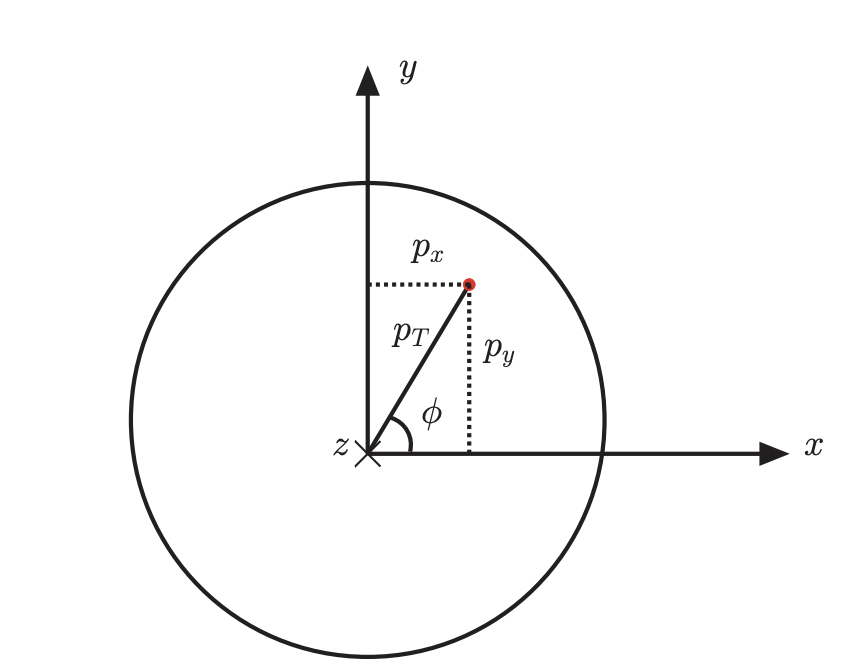
\includegraphics[width=\textwidth]{Figures/atlas/transverse_plane.png}
        \caption{Transverse plane of detector}
        \label{fig:transverse_plane}
    \end{subfigure}
    \hfill
    \begin{subfigure}{.45\textwidth}
        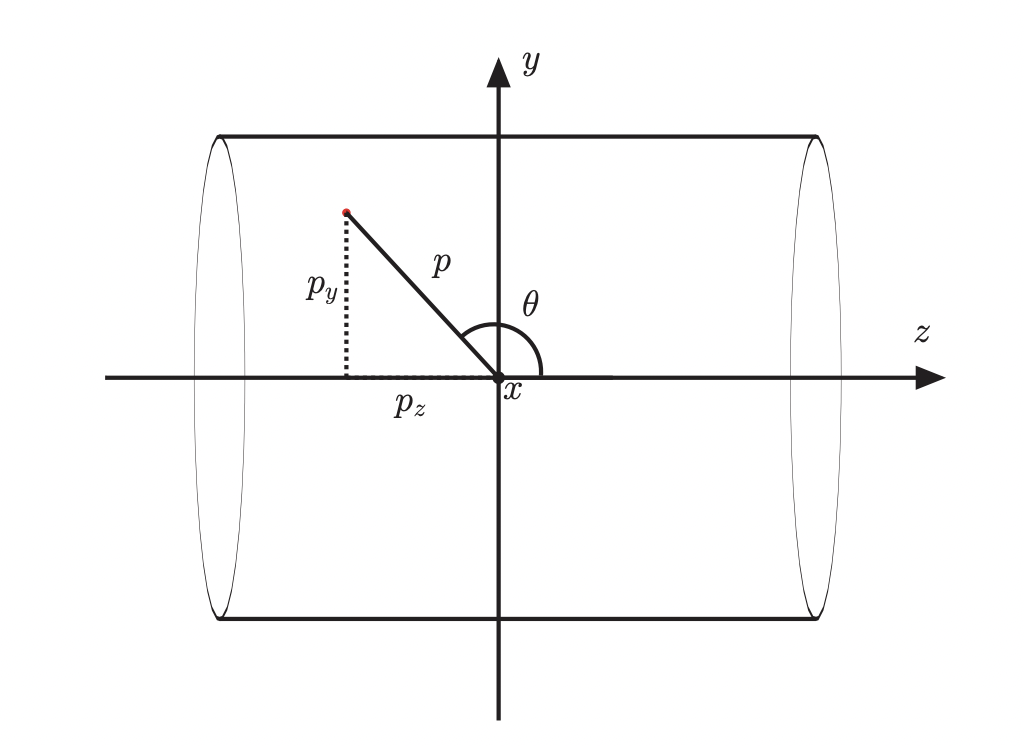
\includegraphics[width=\textwidth]{Figures/atlas/longitudal_plane.png}
        \caption{Longitudal plane of detector}
        \label{fig:longitudal_plane}
    \end{subfigure}
    \hfill
    \caption[ATLAS detector longitudal and azimuthal diagrams]{Spherical coordinate definitions with the azimuthal and polar angles $\phi$ and $\theta$. Here figure \ref{fig:transverse_plane} of the transverse plane shows the z-axis
     into the paper, where as figure \ref{fig:longitudal_plane} of the longitudal plane shows the positive x-axis going out of the paper. Source \href{https://www.duo.uio.no/bitstream/handle/10852/37785/thesis_clean_embedded.pdf?sequence=2&isAllowed=y}{here}. Accessed 16.03.23 }
    \label{fig:long_trans_plane}
\end{figure}

In figure \ref{fig:long_trans_plane} the kinematic variables for proton-proton collisions are described by the energy, rest mass 
and momentum, given as E, m, and $\textbf{p} = (p_x, p_y, p_z)$ respectively. As the particles move with very high energy, we will 
use the relativistic 4 momentum\footnote{In special relativity, 4 momentum is used as both energy and momentum are conserved, and 
thus by creating the 4 momentum, you achieve a Lorentz invariant quantity\cite{Thomson:2013zua}. }, given as $\textbf{P} = (E, \textbf{p})$. We also have that 
\begin{equation*}
    \gamma = \frac{1}{\sqrt{1-\beta^2}},
\end{equation*}
where $\gamma$ is the Lorentz factor, and $\beta = \frac{v}{c}$, which gives us the following definitions for energy $E = \gamma m$ and momentum $\textbf{p} = \beta\gamma m$\cite{Gramstad:1631043}. 
From this we can derive the energy momentum formula:

\begin{align*} 
    \textbf{p}^2 &= \beta^2\gamma^2m^2  \\ 
    \textbf{p}^2 + m^2 &=  m^2(\beta^2\gamma^2 + 1) \\
    \textbf{p}^2 + m^2 &= m^2\gamma^2 \\
    \textbf{p}^2 + m^2 &= E^2
\end{align*}

\begin{equation}\label{eq:energy_momentum}
    E = \sqrt{p^2 + m^2}.
\end{equation}

It can be shown that the phase space of a particle is given by\cite{green_highpt}:

\begin{equation}\label{eq:phase_space}
    d\textbf{p} = dp_xdp_ydp_z = p^2dpd\Omega = dp_zp_Tdp_Td\phi,
\end{equation}

where $p_z$ is the momentum along the beam direction, $p_T$ is the projected momentum on the transverse plane, 
and $\Omega$ is the solid angle. An analog to the relativistic longitudal velocity is the rapidity y. To define this 
we have that the relativistic generalization of equation \ref{eq:phase_space} is given by:
\begin{equation*}
    d^4p\delta (E^2 - p^2 - m^2) = d\textbf{p}\frac{1}{E} = p_T dp_Td\phi dy, \, \, dy = \frac{dp_z}{E}.
\end{equation*}

Using the fact that $p = \sqrt{p_T^2 + p_z^2}$ and equation \ref{eq:energy_momentum} we can integrate $dy$ to get the rapidity:

\begin{equation*}
    \int dy = \int \frac{dp_z}{\sqrt{p_T^2 + p_z^2 + m^2}}
\end{equation*}

\begin{equation}
    y = \cosh^{-1}\left( \frac{E}{\sqrt{p_T^2 + m^2}}\right)
\end{equation}

For particles with little to no mass relative to the transverse momentum, we have that $p_T^2 + m^2 \approx p_T^2$ 
where $p_T = E\sin{(\theta)}$, which gives us the following relations:

\begin{equation*}
    \cosh(y) = \frac{1}{\sin(\theta)},
\end{equation*}
\begin{equation*}
    \sinh(y) = \frac{1}{\tan(\theta)},
\end{equation*}
\begin{equation*}
    \tanh(y) = \cos(\theta).
\end{equation*}

which can be used to show that $e^{-y} = \tan{\frac{\theta}{2}}$. From this we define the pseudorapidity $\eta$ as:
\begin{equation}
    \eta = -\ln{\left( \tan{\frac{\theta}{2}}\right)},
\end{equation}
which is, in the relativistic limit, the same as the rapidity y. A useful property of the pseudorapidity is that 
the phase space of a single particle is uniformly distributed for both $\eta$ and $\phi$, making them good features 
to compare overlap between SM MC and ATLAS data\cite{Gramstad:1631043}. 
\subsection*{Data collection}

\begin{figure}[H]
    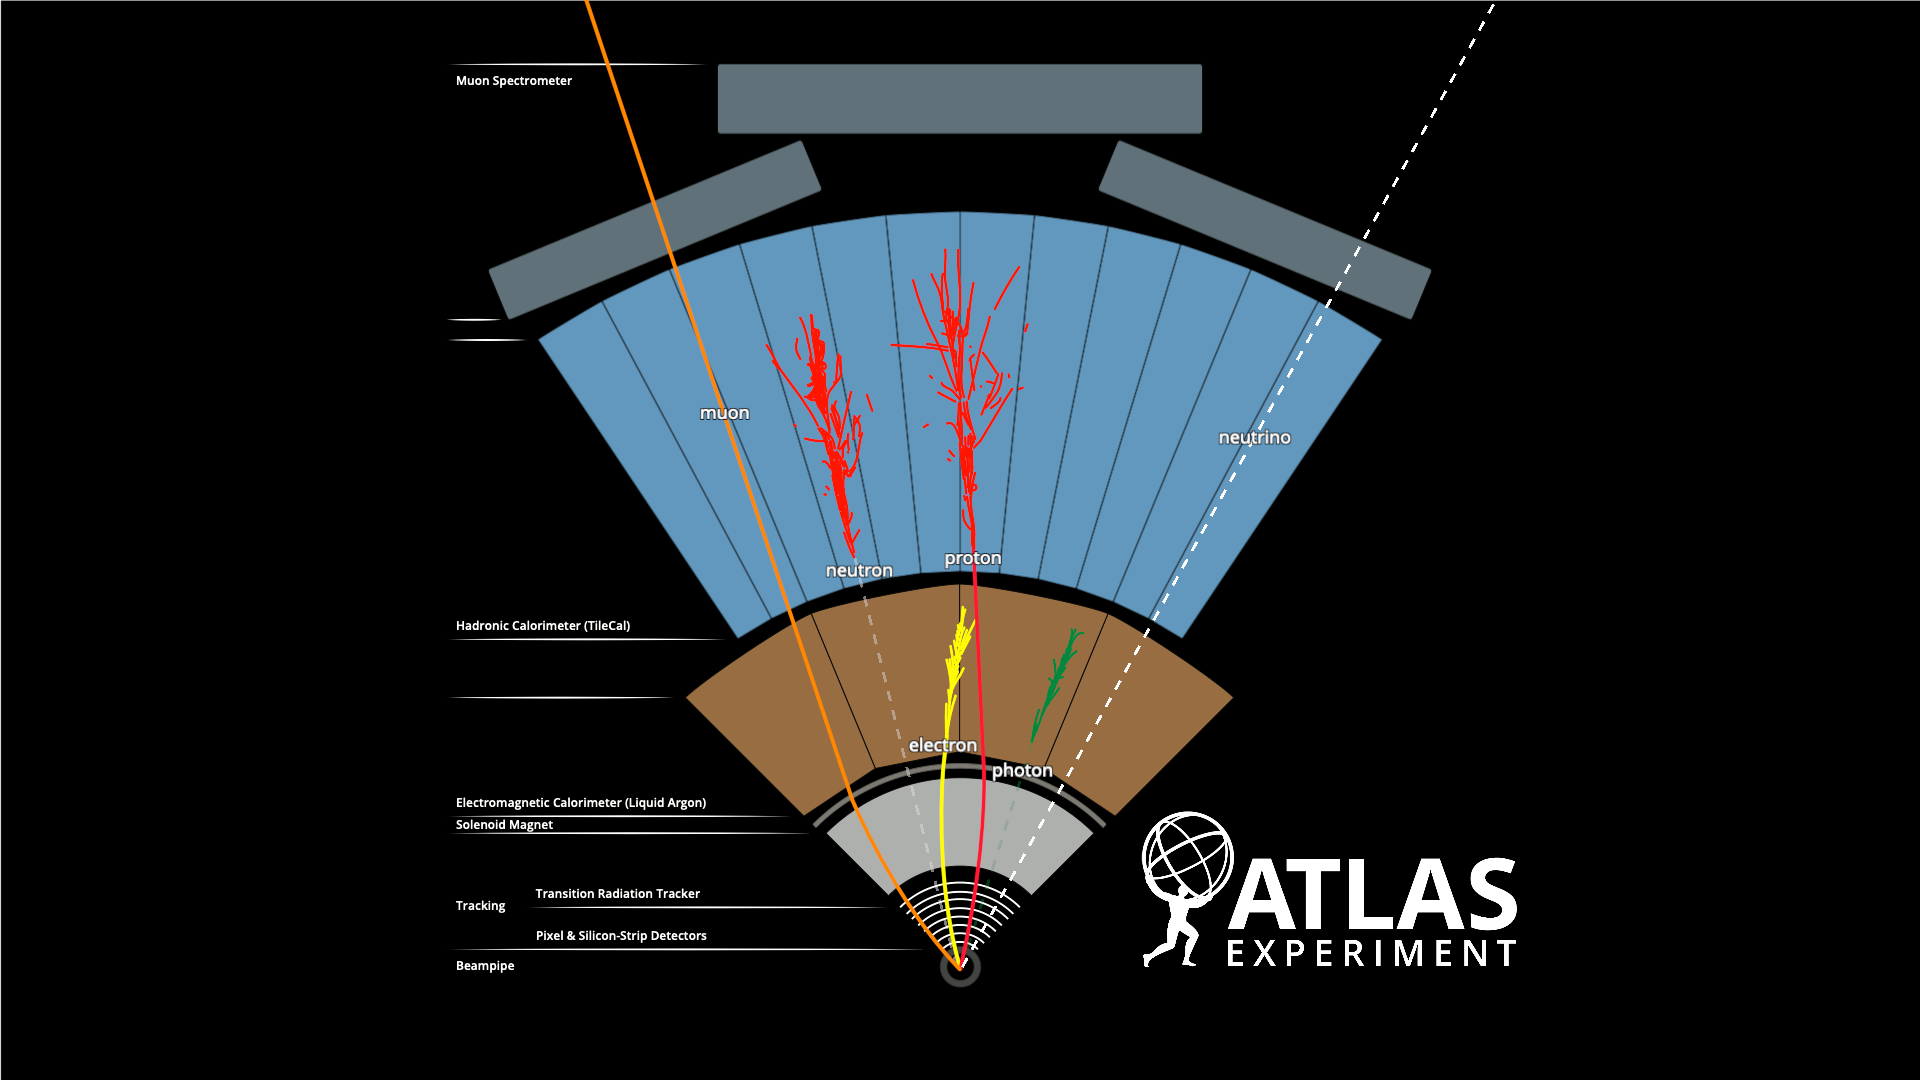
\includegraphics[width=\linewidth]{Figures/atlas/ATLAS Detector Schematic black particles.png}
    \caption[Detector tracking of particles]{Figure describing how particles are detected at ATLAS, fetched from \href{https://cds.cern.ch/record/2770815}{	ATLAS detector slice (and particle visualisations)}, by Sascha Mehlhase \cite{Mehlhase:2770815} . }
    \label{fig:atlas_particle_detect}
\end{figure}

The features used in this analysis are computed with or fetched from the features from the 
detector itself. Such features include the momentum, energy, angles etc., 
all of which are either directly measured or computed based on the measurements in the 
detector. In figure \ref{fig:atlas_particle_detect} a visualization shows how
different particles move through the detector and how they are detected. For example, 
energy deposits are measured using calorimeters, and the different particles 
have calorimeters specially designed for them. Charged particles leave tracks in the 
inner tracking device. Thus, electrons leaves tracks in the inner tracker and deposits energy 
in the elctromagnetic calorimeter, the muons leaves tracks in the inner detector and 
deposits energy in the muon detector. The photons only deposits energy in the electromagnetic 
calorimeter. Hadrons like protons and neutrons deposits energy in the electromagnetic and 
hadronic calorimeters, and charged hadrons also leaves tracks in the inner tracker. This is 
shown in figure \ref{fig:atlas_particle_detect}.\par

The ATLAS detector have a few thousand selection stages before the data is stored. 
In order to reach the highest intensity of collisions, the LHC accellerates
packets of around $10^{11}$ protons, and collides them at a rate of 25 nanoseconds, 
yeilding a collision rate of 40 MHz\cite{Wang:2707056}. \cite{Bernius:2707054}



\subsubsection*{Data preparation}
During datagathering at the ATLAS detector, triggers on the hardware and software level select out the events that are of most interest. On the order of $99 \%$ or
 more of the recorded events are discarded, with about 1 in 40000 events being accepted, as the amount of recorded events simply as too high to realistically analyse. Also, a lot of the events are of no 
 interest for new physics analysis anyway as they for example might have too little energy. Once the trigger selection is done, the data is reconstructed. This means that the objects
 in the recorded events are through software algorithms reconstructed into particles, jets, photons etc. The reconstruction is done based on the tracks and measurements
 in the detector, but it is not perfect, and can lead to fake leptons or jets. By fake, it is meant that an object might look like a lepton but is in reality a jet or vice versa\cite{Gillam:2015kta}.
 Once the reconstruction is done, further slimming of the n-tuples are done. Derivations are slimmings of the n-tuples where the selection of events are further reduced 
 to match the needs of the different analysis groups. \par 
The SM MC go through parts of the same process. These events are first generated and then run through the detector to simulate actual events. Once that is done, the events
 can be reconstructed and go through derivations just like the pp-collision data, to be used in analysis. 

\begin{figure}[H]
    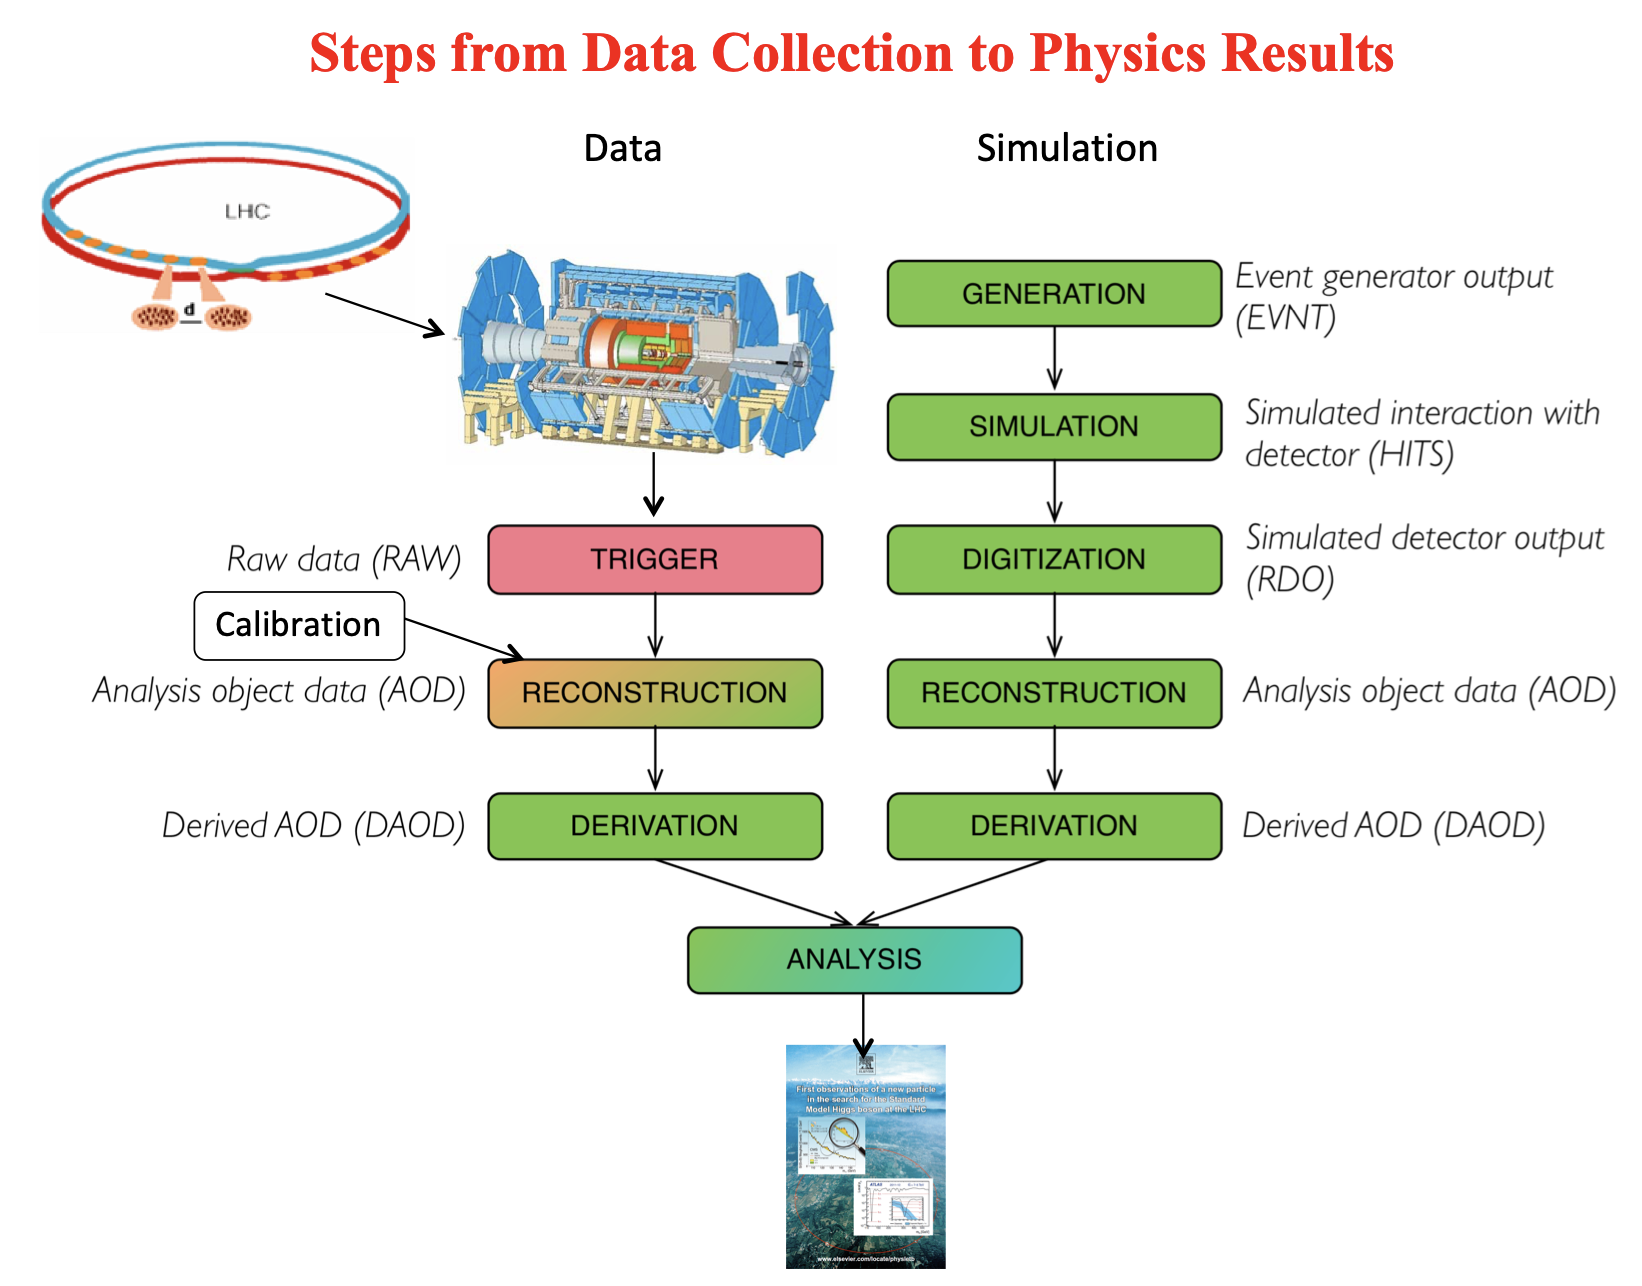
\includegraphics[width=\linewidth]{Figures/atlas/data_col_phys.png}
    \caption[Steps from data collection to physics results]{Figure describing the steps to take for data collection at ATLAS, fetched from \href{https://indico.cern.ch/event/1159574/timetable/?view=standard}{Hybrid ATLAS Induction Day + Software Tutorial workshop}, part
    \href{https://indico.cern.ch/event/860971/contributions/3672974/attachments/1972049/3280896/Atlas_computing_data_preparation_jan20.pdf}{Computing and Data preparation}, 
    held by S.M Wang \cite{Wang:2707056} . }
    \label{fig:atlas_data_col_phys}
\end{figure}


\subsubsection*{Jets}
Photons and electrons are detected in the electromagnetic calorimeter, and are easy to track and detect as they 
separate easily. Quarks, however, are bound by QCD and thus cannot be seperated as individual 
particles. An illustration of how quarks and gluons materialise as jets during a proton-proton 
collision is shown below in figure \ref{fig:cms_jets}.

\begin{figure}[H]
    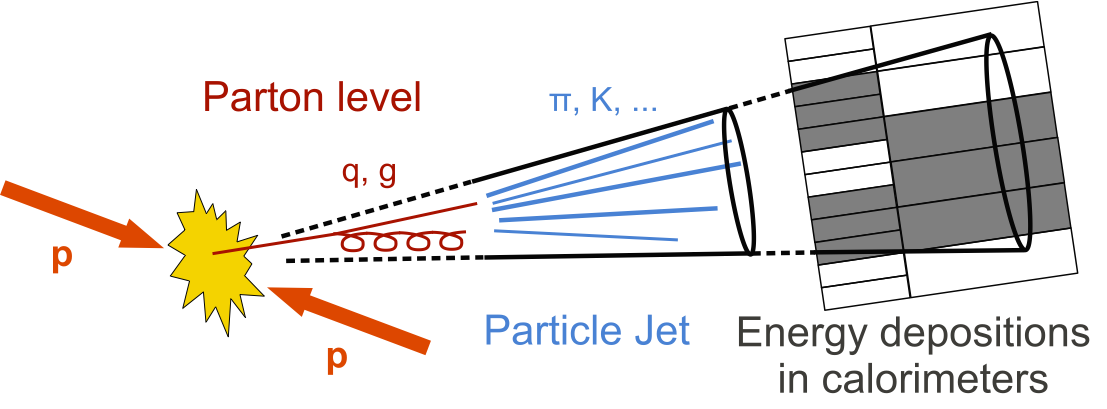
\includegraphics[width=\linewidth]{Figures/atlas/cms_Sketch_PartonParticleCaloJet.png}
    \caption[Jet produciton from pp-collisions to detector]{Figure describing how quarks and gluons are treated in the detector, and thus why we name them jets, fetched from \href{https://cms.cern/sites/default/files/field/image/Sketch_PartonParticleCaloJet.png}{the CMS webpage}. }
    \label{fig:cms_jets}
\end{figure}

In a proton-proton collision, the quarks and gluons forms stable or unstable hadrons such that the color confinement\footnote{Add link to a source or explanation for this.} is upheld. These then 
decay to other stable hadrons that can be tracked, and these tracks are called jets. This is particularly difficult because one wants to isolate which hadrons came from  the original quark in the 
Feynman diagram. Another point to make is that some quarks are of higher interest than others. For example, the b jet, coming from a b quark, is a good indicator for certain processes, 
thus identifying suchs particles is of huge interest. 